% ----------------------------------------------------
% DAB Processing
% ----------------------------------------------------
\documentclass[class=report,11pt,crop=false]{standalone}
% Page geometry
\usepackage[a4paper,margin=25mm,top=25mm,bottom=25mm]{geometry}

% Font choice
\usepackage{lmodern}

% Use IEEE bibliography style
\bibliographystyle{IEEEtran}

% Line spacing
\usepackage{setspace}
\setstretch{1.20}

% Ensure UTF8 encoding
\usepackage[utf8]{inputenc}

% Language standard (not too important)
\usepackage[english]{babel}

% Skip a line in between paragraphs
\usepackage{parskip}

% For the creation of dummy text
\usepackage{blindtext}

% Math
\usepackage{amsmath}

% Header & Footer stuff
\usepackage{fancyhdr}
\pagestyle{fancy}
\fancyhead{}
\fancyhead[R]{\nouppercase{\rightmark}}
\fancyfoot{}
\fancyfoot[C]{\thepage}
\renewcommand{\headrulewidth}{0.0pt}
\renewcommand{\footrulewidth}{0.0pt}
\setlength{\headheight}{13.6pt}

% Page geometry
\usepackage[a4paper,top=25mm,bottom=25mm]{geometry}

% Epigraphs
\usepackage{epigraph}
\setlength\epigraphrule{0pt}

% Hyperlinks & References
\usepackage{hyperref}
\hypersetup{
    colorlinks=true,
    linkcolor=blue,
    filecolor=blue,      
    urlcolor=blue,
    citecolor=blue,
}
\urlstyle{same}

% Automatically correct front-side quotes
\usepackage[autostyle=false, style=american]{csquotes}
\MakeOuterQuote{"}

% Graphics
\usepackage{graphicx}
\graphicspath{{Images/}{../Images/}}

% Colour
\usepackage{color}
\usepackage[usenames,dvipsnames]{xcolor}

% SI units
\usepackage{siunitx}

% Microtype goodness
\usepackage{microtype}

% Listings
\usepackage{listings}
\definecolor{backgroundColour}{RGB}{250,250,250}
\definecolor{commentColour}{RGB}{73, 175, 102}
\definecolor{identifierColour}{RGB}{196, 19, 66}
\definecolor{stringColour}{RGB}{252, 156, 30}
\definecolor{keywordColour}{RGB}{50, 38, 224}
\definecolor{lineNumbersColour}{RGB}{127,127,127}
\lstset{ 
  language=Matlab,
  captionpos=b,
  backgroundcolor=\color{backgroundColour},
  basicstyle=\footnotesize,        % the size of the fonts that are used for the code
  breakatwhitespace=false,         % sets if automatic breaks should only happen at whitespace
  breaklines=true,                 % sets automatic line breaking
  postbreak=\mbox{\textcolor{red}{$\hookrightarrow$}\space},
  commentstyle=\color{commentColour},    % comment style
  identifierstyle=\color{identifierColour},
  stringstyle=\color{stringColour},
   keywordstyle=\color{keywordColour},       % keyword style
  %escapeinside={\%*}{*)},          % if you want to add LaTeX within your code
  extendedchars=true,              % lets you use non-ASCII characters; for 8-bits encodings only, does not work with UTF-8
  frame=single,	                   % adds a frame around the code
  keepspaces=true,                 % keeps spaces in text, useful for keeping indentation of code (possibly needs columns=flexible)
  morekeywords={*,...},            % if you want to add more keywords to the set
  numbers=left,                    % where to put the line-numbers; possible values are (none, left, right)
  numbersep=5pt,                   % how far the line-numbers are from the code
  numberstyle=\tiny\color{lineNumbersColour}, % the style that is used for the line-numbers
  rulecolor=\color{black},         % if not set, the frame-color may be changed on line-breaks within not-black text (e.g. comments (green here))
  showspaces=false,                % show spaces everywhere adding particular underscores; it overrides 'showstringspaces'
  showstringspaces=false,          % underline spaces within strings only
  showtabs=false,                  % show tabs within strings adding particular underscores
  stepnumber=1,                    % the step between two line-numbers. If it's 1, each line will be numbered
  tabsize=2,	                   % sets default tabsize to 2 spaces
  %title=\lstname                   % show the filename of files included with \lstinputlisting; also try caption instead of title
}

% Caption stuff
\usepackage{caption}
\usepackage{subcaption}

\makenoidxglossaries

\newacronym{radar}{RADAR}{Radio Detection and Ranging}
\newacronym{dab}{DAB}{Digital Audio Broadcasting}
\newacronym{fm}{FM}{Frequency Modulation}
\newacronym{am}{AM}{Amplitude Modulation}
\newacronym{fdm}{FDM}{Frequency Division Multiplexing}
\newacronym{ofdm}{OFDM}{Orthogonal Frequency Division Multiplexing}
\newacronym{cofdm}{COFDM}{Coded Orthogonal Frequency Division Multiplexing}
\newacronym{dvbt2}{DVB–T2}{Digital Video Broadcasting — Second Generation Terrestrial}
\newacronym{em}{EM}{electromagnetic}
\newacronym{icasa}{ICASA}{Independent Communications Authority of South Africa}
\newacronym{ioo}{IOO}{Illuminators of Opportunity}
\newacronym{pr}{PR}{Passive Radar}
\newacronym{qpsk}{QPSK}{Differential Quadrature Phase-Shift Keying}
\newacronym{dqpsk}{DQPSK}{Differential Quadrature Phase-Shift Keying}
\newacronym{etsi}{ETSI}{European Telecommunications Standards Institute}
\newacronym{psk}{PSK}{Phase Shift Keying}
\newacronym{ask}{ASK}{Amplitude-Shift Keying}
\newacronym{fsk}{FSK}{Frequency-Shift Keying}
\newacronym{iq}{IQ}{In-phase and Quadrature}
\newacronym{prs}{PRS}{Phase Reference Symbol}
\newacronym{dft}{DFT}{Discrete Fourier Transform}
\newacronym{fft}{FFT}{Fast Fourier Transform}
\begin{document}
\ifstandalone
\tableofcontents
\fi
% ----------------------------------------------------
\chapter{Digital Audio Broadcasting: Processing Chain Design}
\epigraph{Nobody can build you the bridge over which you must cross the river of life, nobody but you alone.}%
    {\emph{---Friedrich Nietzsche}}
% ----------------------------------------------------

This chapter details the core design component of the project: a \gls{dab} processing chain. While the broader context of this report falls within the realm of \gls{pr}, the fundamental task at hand was to demodulate and remodulate a given \gls{dab} signal, in order to create a perfect reference signal of given recorded data. Fortunately, as outlined in the previous chapter, not all of the intricacies of the \gls{dab} standard were required to be understood or even considered for integration into a passive radar chain.

The design of the chain involved studying the \gls{dab} standard document from the \gls{etsi}~\cite{dabstandard}, as well as using a reference signal which was known to be perfectly modulated for initial testing. For some functionality, real-world data was also used for design and testing. For the sake of simplicity, the entire chain---including all the dimensions shown in this chapter---was designed around \gls{dab} Mode 1. Nonetheless, altering the chain for implementation with other modes will be trivial. All MATLAB functions were designed with a \texttt{dab\_mode} input, if necessary, to allow for easy changes in future designs. Note, however, that this mode input parameter is not shown in any of the upcoming diagrams.

\section{Overview}
Within the \gls{dab} processing chain, three main functional blocks were identified: pre-processing, demodulation, and remodulation. The first block reads in a \gls{dab} recording of \gls{iq} data saved as a binary file, and outputs a single \gls{dab} frame from this file. This frame can then be input to the demodulate block, which extracts the \gls{dab} data from it. This data is not the decoded information from the \gls{dab} recording---such as the audio signal---rather, it is simply an extracted bitstream. This bitstream can then be perfectly reconstructed as a \gls{dab} frame, by the remodulate block. A diagrammatic overview of this chain is given in Figure~\ref{fig:BD_Overview_All}.

\begin{figure}[htbp]
  \centering
  \captionsetup{type=figure}
  \def\svgwidth{\linewidth}
  {\setstretch{0.7} % Line spacing
      \input{../Images/BD_Overview_All-embed.pdf_tex}}
  \caption{Block diagram showing entire DAB processing chain}
  \label{fig:BD_Overview_All}
\end{figure}

Notice in the figure that each of the aforementioned blocks---the pre-process, demodulate, and remodulate blocks---was created from a collection of smaller sub-blocks. These sub-blocks were designed to perform simpler tasks individually, and were written as relatively short MATLAB functions. This atomic-function approach had a host of benefits for the design, debugging, and validation of the chain, and added layers of abstraction for the larger system.

Each of the three blocks will be unpacked in the sections that follow this one, with subsections dedicated to the relevant sub-blocks.

\section{Pre-processing \label{sect:dab-proc_preprocessing}}
\subsection{Overview}
The pre-processing chain was designed to read in an \gls{iq} data file, synchronize it appropriately, and extract a single frame from it. Note that in an actual \gls{pr} system---where this \gls{dab} processing chain would be only a small part of a larger chain---this block would be markedly different. If nothing else, a real-world chain would probably stream the \gls{iq} data, rather than read it from a pre-recorded file. Moreover, a real chain might process several \gls{dab} frames at once. However, such details are largely context-specific, and it would be superfluous to include every use-case in this report. Importantly, the other two blocks---used to demodulate and remodulate---would mostly remain the same in various other scenarios. Thus, to make matters simpler, the pre-processing block was designed to be straightforward: to read in data and extract a single frame. That is not to say the block is trivial, and there were some important design decisions made for it.

The pre-processing block has four key stages: reading in \gls{iq} data from a binary file, resampling this data if necessary, detecting the location of the \gls{prs} and thus synchronizing the recording, and then extracting a \gls{dab} frame accordingly. This pipeline is shown graphically in Figure~\ref{fig:BD_Preprocess_All}.

\begin{figure}[htbp]
    \centering
    \captionsetup{type=figure}
    \def\svgwidth{\linewidth}
    {\setstretch{0.7} % Line spacing
        \input{../Images/BD_Preprocess_All-embed.pdf_tex}}
    \caption{Block diagram showing preprocessing section of processing chain}
    \label{fig:BD_Preprocess_All}
\end{figure}

\subsection{Reading IQ data from file \label{subsect:dab-proc_iq-read}}
The first sub-block is called \texttt{iq\_read}, and, as mentioned previously, would likely be very different in a real \gls{pr} chain. Nonetheless, here it reads in a \gls{dab} recording from a binary file, and outputs so-called "raw" \gls{iq} data. No changes are made to this data in this function, and it essentially just abstracts MATLAB's file-handling functionality conveniently.

As a minor note, one must remember that a \gls{dab} recording contains \gls{iq} data, which is complex-valued. Since a binary file cannot store such a datatype, it will usually be stored as pairs of numbers. To read this correctly in MATLAB, one can use the simple code shown in Listing~\ref{code:iq_read}.

\begin{lstlisting}[caption={Creating a complex data array with the values read from a binary file},label={code:iq_read}]
iq_data_raw = data_from_file(1:2:end) + 1j*data_from_file(2:2:end);
\end{lstlisting}

Though it is not shown in the pre-processing block diagrams, the MATLAB function for \texttt{iq\_read} also included some other input parameters for convenience, including the data-type of the binary file, the offset to skip in the file's data, the number of frames to read, and so on.

A perfect \gls{dab} recording that would be output from the \texttt{iq\_read} function is shown in Figure~\ref{fig:plots/perfect-dab-signal}, showing a handful of \gls{dab} frames. Notice the separation of successive frames by the distinct null symbols.

\begin{figure}[htbp]
  \centering
  \captionsetup{type=figure}
  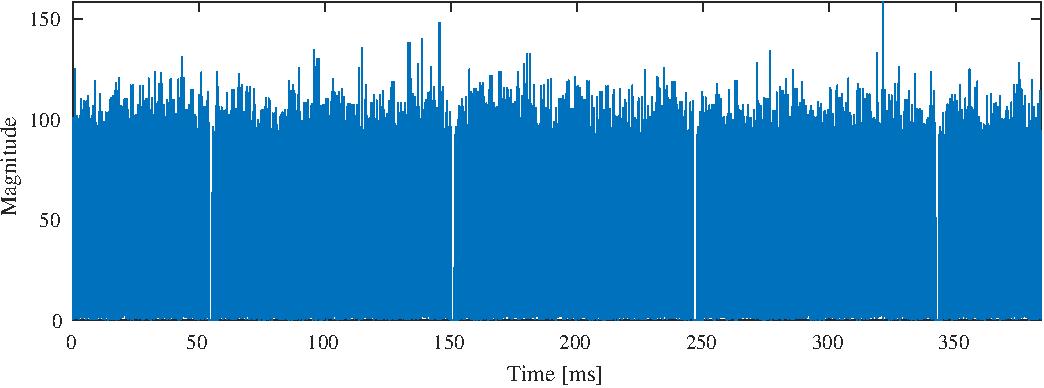
\includegraphics[width=\linewidth]{plots/perfect-dab-signal.pdf}
  \caption{Time-domain plot of a handful of frames of a perfect \gls{dab} signal}
  \label{fig:plots/perfect-dab-signal}
\end{figure}

\subsection{Resampling IQ data \label{subsect:dab-proc_iq-resample}}
In order for one to utilise the \gls{fft} to demodulate an \gls{ofdm} symbol, certain requirements must be met. Recall that the window for a single symbol, notated as \(T_u\), is 2048 samples for \gls{dab} Mode 1. This means that a 2048-point \gls{fft} must be used, with a resulting 2048 points in the frequency domain. Recall also that \gls{ofdm} has a strict requirement for the spacing between adjacent carriers---\(1 \si{\kilo \hertz}\) for \gls{dab} Mode1. Notice, then, if the sample rate for the original signal is precisely set at \(F_s = 2.048 \si{\mega \hertz}\), for \gls{dab} Mode 1, then the bins from the \gls{fft} will be perfectly aligned on the \gls{ofdm} carriers---enabling proper demouldation.

However, in a real-world scenario, the desired sampling rate might not necessarily be used in the receiver. Thus, in such a situation, the \gls{iq} data must be resampled. Consider an original sampling rate of \(F_s\), a desired sampling rate of \(\tilde{F_s} = 2.048 \si{\mega \hertz}\), with \(F_s \ne \tilde{F_s}\), and with
\begin{equation}
  \frac{\tilde{F_s}}{F_s} = \frac{P}{Q}
\end{equation}
where \(P\) and \(Q\) are integers---preferably chosen such that \(P/Q\) is in its most reduced fractional form. Resampling, then, is equivalent to upsampling by a factor of \(P\), and thereafter downsampling by a factor of \(Q\).

Fortunately, MATLAB provides a neat abstraction of this process with the \texttt{resample(X, P, Q)} function, where \(X\) is a uniformly sampled signal, and \(P\) and \(Q\) are as defined above.

% -----------------
\subsection{Frame Synchronization via Phase Reference Symbol Detection \label{subsect:dab-proc_prs-detect}}

One of the most important parts of the entire \gls{dab} processing chain is correct synchronization. If the frame that is output from the pre-processing block is misaligned, the entire demodulation process can break due to misalignment of the \gls{ofdm} symbols. It will later be shown how negatively a result is affected by the incorrect alignment of a \gls{dab} frame.

There are two mechanisms built into the \gls{dab} signal for synchronization, namely the \acrfull{ns} and the \acrfull{prs}. As specified in the \gls{dab} standard document~\cite{dabstandard}, the former symbol can be used for coarse synchronization, whereas the latter is used for fine synchronization. Essentially, then, there are two approaches to frame alignment: to locate the approximate beginning of a frame with the \gls{ns} and then finely align the frame with the \gls{prs}, or to use only the \gls{prs} without first coarsely detecting the \gls{ns}.

For each of these detection processes, only a short chunk of the data will be considered at once. Let the length of this window be notated as \(T_w\), and let the interval between successive chunks be called the "advancement" interval, \(T_a\). In order not to skip any sections of the signal, it is clear that,
\begin{equation}
  T_a \le T_w
\end{equation}

Graphically, the frame synchronization situation is depicted in Figure~\ref{fig:sliding-window-illustration}.

\begin{figure}[htbp]
  \centering
  \captionsetup{type=figure}
  \def\svgwidth{\linewidth}
  {\setstretch{0.7} % Line spacing
      \input{../Images/sliding-window-illustration.pdf_tex}}
      \caption{Depiction of sliding window across a recorded \gls{dab} signal}
      \label{fig:sliding-window-illustration}
\end{figure}


Recall that the Null Symbol is a period during which all \gls{ofdm} carriers are turned off. In order to detect this symbol, one can, for example, look for a significant drop in the average power of the incoming signal, \(P_x\):
\begin{equation}
  P_x = \frac{1}{T} \cdot \sum^{T-1}_{n=0} \Big| x[n] \Big|^2
\end{equation}
where \(x[n]\) is the sampled signal, and \(T\) is the length of the chunk of signal to be considered---likely set to \(T_\textrm{null}\), the length of the Null Symbol.

The \gls{prs}, on the other hand, can be detected via a Matched Filtering process, which is essentially a time-domain correlation. Conceptually, this filter, \(H(\Omega)\), is designed as:
\begin{equation}
  H(\Omega) = R^*(\Omega)
\end{equation}
where \(R^*(\Omega)\) is the conjugate of the continuous-time Fourier transform of the \gls{prs}. Of course, since the system is implemented digitally, the filter must be defined discretely,
\begin{equation}
  \mathbf{H} = \mathbf{R}^* = \mathrm{DFT} \{ r[n] \}^*
\end{equation}

Then, the output of the filter in the Fourier domain, \(\mathbf{Y}\), can be calculated via a simple Hadamard product:
\begin{equation}
  \mathbf{Y} = \mathbf{H} \odot \mathbf{X}
\end{equation}

Notice that for each of these symbol detection processes, only a certain chunk of the original signal is considered at once---there is a window applied. Thus there is a decision on the so-called "Window Advancement Interval"---the interval between successive windows for the detection process. This is depicted in Figure~\ref{fig:sliding-window-illustration}.

At a maximum, this interval should be as long as a window itself, in order not to skip any sections of the original signal. Alternatively, for a variety of reasons, the interval may be shorter than the window length. Two possibilities for the Window Advancement Interval are shown in figure~\ref{fig:matched-filter-sliding-window-advance}.

\begin{figure}[htbp]
  \centering
  \captionsetup{type=figure}
  \def\svgwidth{\linewidth}
  {\setstretch{0.7} % Line spacing
      \input{../Images/matched-filter-sliding-window-advance.pdf_tex}}
      \caption{Depiction of two Window Advancement Intervals alongside a \gls{dab} signal}
      \label{fig:matched-filter-sliding-window-advance}
\end{figure}

To simplify the processing chain, the frame synchronization was done using only the phase reference symbol.

% For \gls{dab} Mode 1, the \gls{prs} has a length of 2048 samples. Thus, in order to detect the symbol within an incoming \gls{dab} signal, one can use a Matched Filter, designed around the \gls{prs}. This Matched Filter will naturally have 2048 samples, and so a sliding window of 2048 samples must also be used. The most straightforward way of doing this would be to look at chunks of the incoming signal, in steps of 2048. This is depicted in Figure~\ref{fig:matched-filter-sliding-window}.

\begin{figure}[ht]
    \centering
    \captionsetup{type=figure}
    \begin{minipage}{.6\linewidth}
      \begin{algorithm}[H]
        \caption{How to write algorithms \label{alg:test}}

        \SetAlgoLined
        
        \KwData{this text}
        
        \KwResult{how to write algorithm with \LaTeX2e }
        initialization\;
        
        \While{not at end of this document}{
          read current\;
          \eIf{understand}{
            go to next section\;
            current section becomes this one\;
          }{
            go back to the beginning of current section\;
          }
        }

      \end{algorithm}
    \end{minipage}
\end{figure}

An important question when integrating the \gls{dab} processing chain into a larger \gls{pr} system is the regularity of frame synchronization. Ideally, one would only need to synchronize once, if the clock of the transmitter and receiver are perfectly accurate. Unfortunately, in real scenarios, there are a host of unwanted effects, including clock drift, that may cause synchronization errors over time. The other extreme is to synchronize on every frame---which is possible because every frame is preceded by both a Null Symbol and a \gls{prs}. However, this may prove to be too computationally expensive. Naturally, fixed rules cannot be set for this decision, and are largely context-specific. Further details are thus omitted here.

\subsection{Frame Extraction \label{subsect:dab-proc_frame-extract}}
Once the index of the \gls{prs} has been detected, extracting a frame is trivial, as it simply entails subsetting the original data array. This block and subsection are included for the sake of completeness.


\section{Demodulation \label{sect:dab-proc_demodulate}}
\subsection{Overview}
The purpose of the demodulation block is to extract \gls{dab} "information" from a given frame. This not a \emph{decoder}, as it does not extract any audio signal or similar. Rather, it returns the bitstream with which the \gls{ofdm} carrier waves were modulated. Importantly, this demodulator block is not intended to stand alone, and its output is useless in isolation. Instead, the demodulation and remodulation blocks are designed to operate in tandem, where the output of the demodulate block is the input to the remodulate block. Ultimately, this is all for the purpose of perfectly reconstructing a given \gls{dab} frame, to be used in a \gls{pr} chain.

The demodulation pipeline has six key stages: the \gls{dab} frame is unpacked into a collection of symbols, which is then demultiplexed into \gls{ofdm} carriers, which are then demapped into \gls{dab} data via \gls{dqpsk} demodulation. Thereafter, this \gls{dab} data is interleaved in frequency, snapped to their closest \gls{dqpsk} values, and finally are put through an error-correction algorithm. The overview of this chain is given in Figure~\ref{fig:BD_Demod_All}. Take special note of the nomenclature for the variables before and after each block, as well as their dimensions---provided for \gls{dab} Mode 1.

\begin{figure}[htbp]
    \centering
    \captionsetup{type=figure}
    \def\svgwidth{\linewidth}
    {\setstretch{0.7} % Line spacing
        \input{../Images/BD_Demod_All-embed.pdf_tex}}
    \caption{Block diagram showing demodulation section of processing chain}
    \label{fig:BD_Demod_All}
\end{figure}

The details for each sub-block are given in the following sections.

\subsection{Symbols Unpacking \label{subsect:dab-proc_symbols-unpack}}
The purpose of this function is to split a \gls{dab} frame into its symbols, which can then be demultiplexed and further processed. This sub-block also includes the removal of guard intervals from the symbols, thus extracting only the "useful symbol" component. As a result, the function receives a vector of size \(1\times T_f\), and outputs a matrix of size \(L\times T_u\). Note that
\begin{equation}
  T_f \ne L\times T_u
\end{equation}
since the original frame length, \(T_f\), includes the guard intervals of length \(Tg\), as well as the \gls{ns}. Instead,
\begin{equation}
  T_f = L\times (T_u + T_g) + T_\mathrm{null}
\end{equation}

The symbol unpacking process is depicted graphically in figure~\ref{fig:symbols_unpack}.

\begin{figure}[htbp]
  \centering
  \captionsetup{type=figure}
  \def\svgwidth{\linewidth}
  {\setstretch{0.7} % Line spacing
      \input{../Images/symbols_unpack.pdf_tex}}
  \caption{Illustration of the \texttt{symbol\_unpack} functionality}
  \label{fig:symbols_unpack}
\end{figure}

In MATLAB, the unpacking process is fairly straightforward, with complications only arising in off-by-one errors. Consider the simple code segment in Listing~\ref{code:symbols_unpack} for this functionality.

\begin{lstlisting}[caption={Code used in the \texttt{symbols\_unpack} function}, label={code:symbols_unpack}]
function dab_symbols = symbols_unpack(dab_frame, dab_mode)
  % Pre-allocate space for the result
  dab_symbols = zeros(dab_mode.L, dab_mode.Tu);

  % Start after null & first guard interval
  ii = dab_mode.Tnull + dab_mode.Tg + 1;

  % Iterate through L symbols
  for l = 1:dab_mode.L
      % Read symbol of length Tu
      dab_symbols(l,:) = dab_frame(ii:ii+dab_mode.Tu-1);
      % Jump ahead 1 symbol, incl. guard (Ts = Tu + Tg)
      ii = ii + dab_mode.Ts;
  end
end
\end{lstlisting}

% -------------
\subsection{OFDM Demultiplexing \label{subsect:dab-proc_ofdm-demux}}
With the individual symbols extracted from the \gls{dab} frame, the \gls{ofdm} carriers can then be extracted via a \gls{fft} operation, as explained in the previous chapter. Consider first the case of a single symbol.

\begin{figure}[htbp]
  \centering
  \begin{subfigure}[t]{0.45\textwidth}
    \centering
    \captionsetup{type=figure}
    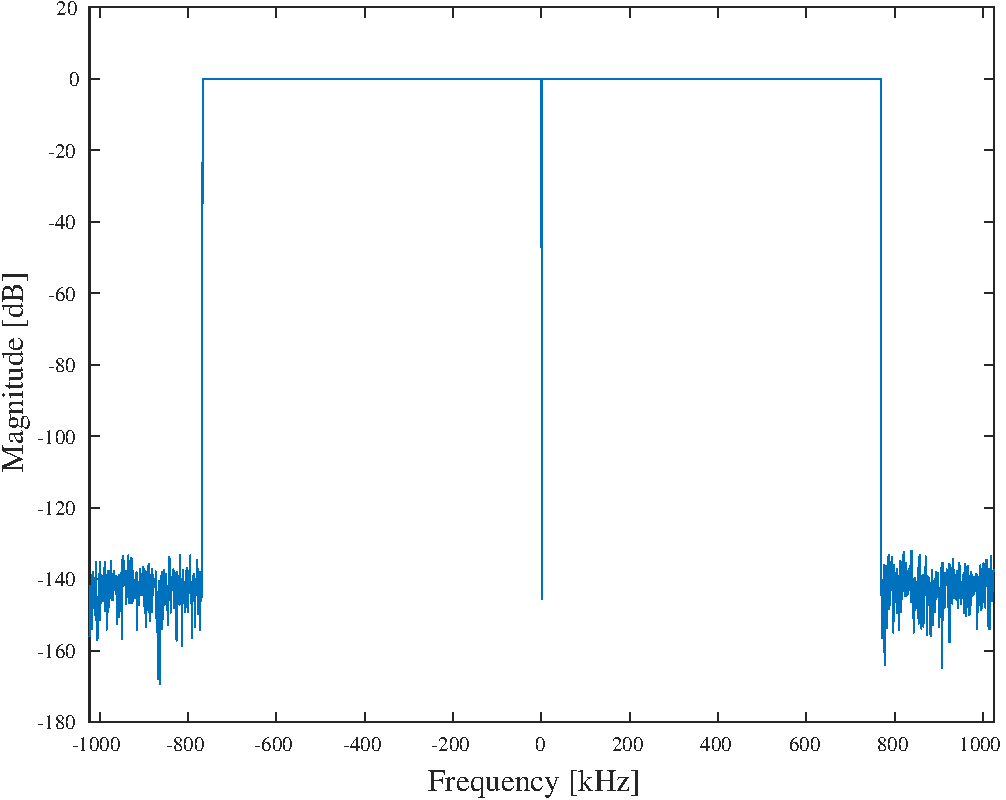
\includegraphics[width=\linewidth]{plots/ofdm-carriers-perfect.pdf}
    \caption{Perfect Data}
    \label{fig:ofdm-carriers-perfect}
  \end{subfigure}%
  ~ 
  \begin{subfigure}[t]{0.45\textwidth}
    \centering
    \captionsetup{type=figure}
    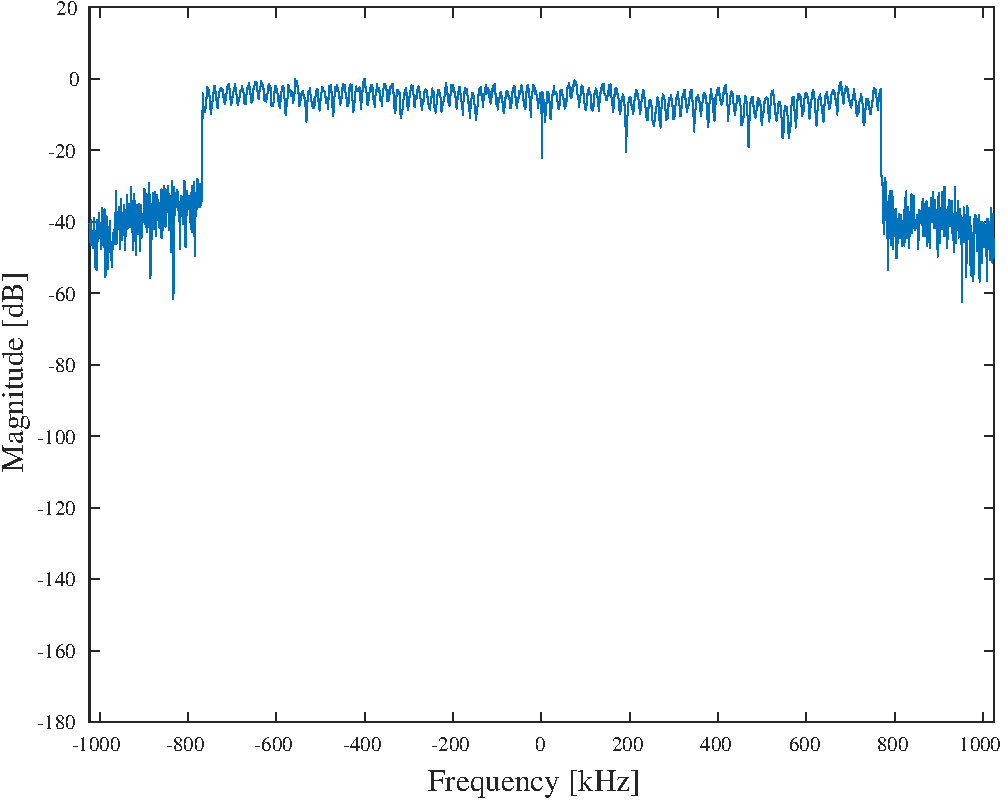
\includegraphics[width=\linewidth]{plots/ofdm-carriers-raw.pdf}
    \caption{Actual Data}
    \label{fig:ofdm-carriers-raw}
  \end{subfigure}
  \caption{Plots showing the magnitude of the \gls{ofdm} carriers for a single \gls{dab} symbol}
  \label{fig:dqpsk_demap_perfect}
\end{figure}

\begin{figure}[htbp]
  \centering
  \captionsetup{type=figure}
  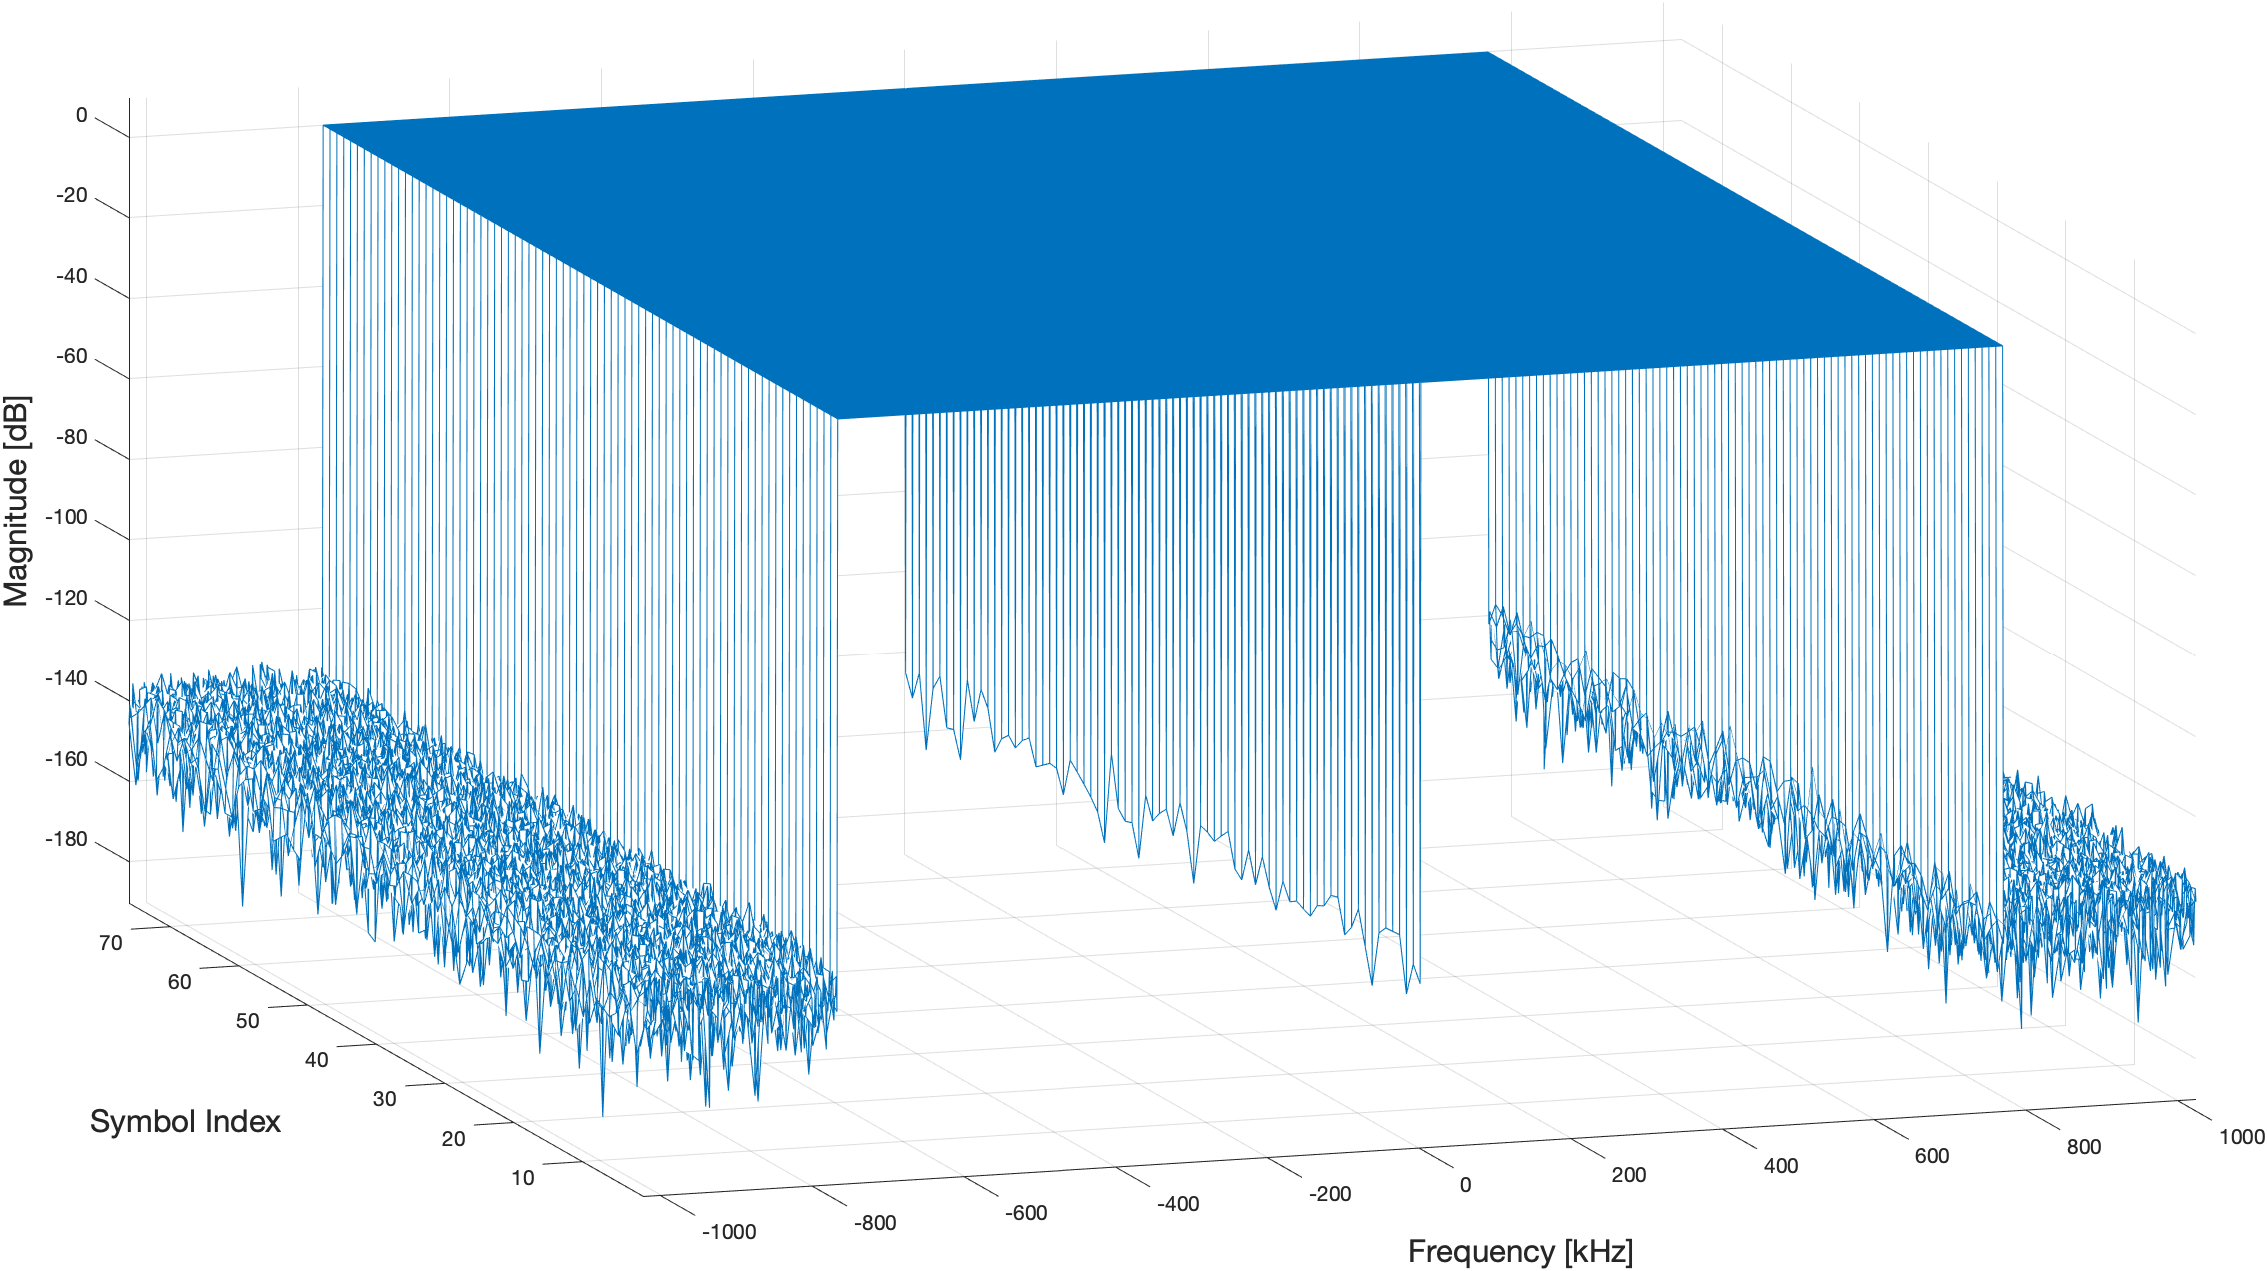
\includegraphics[width=0.9\linewidth]{plots/ofdm-surface-perfect.png}
  \caption{Surface plot}
  \label{fig:ofdm-surface-perfect}
\end{figure}

\begin{figure}[htbp]
  \centering
  \captionsetup{type=figure}
  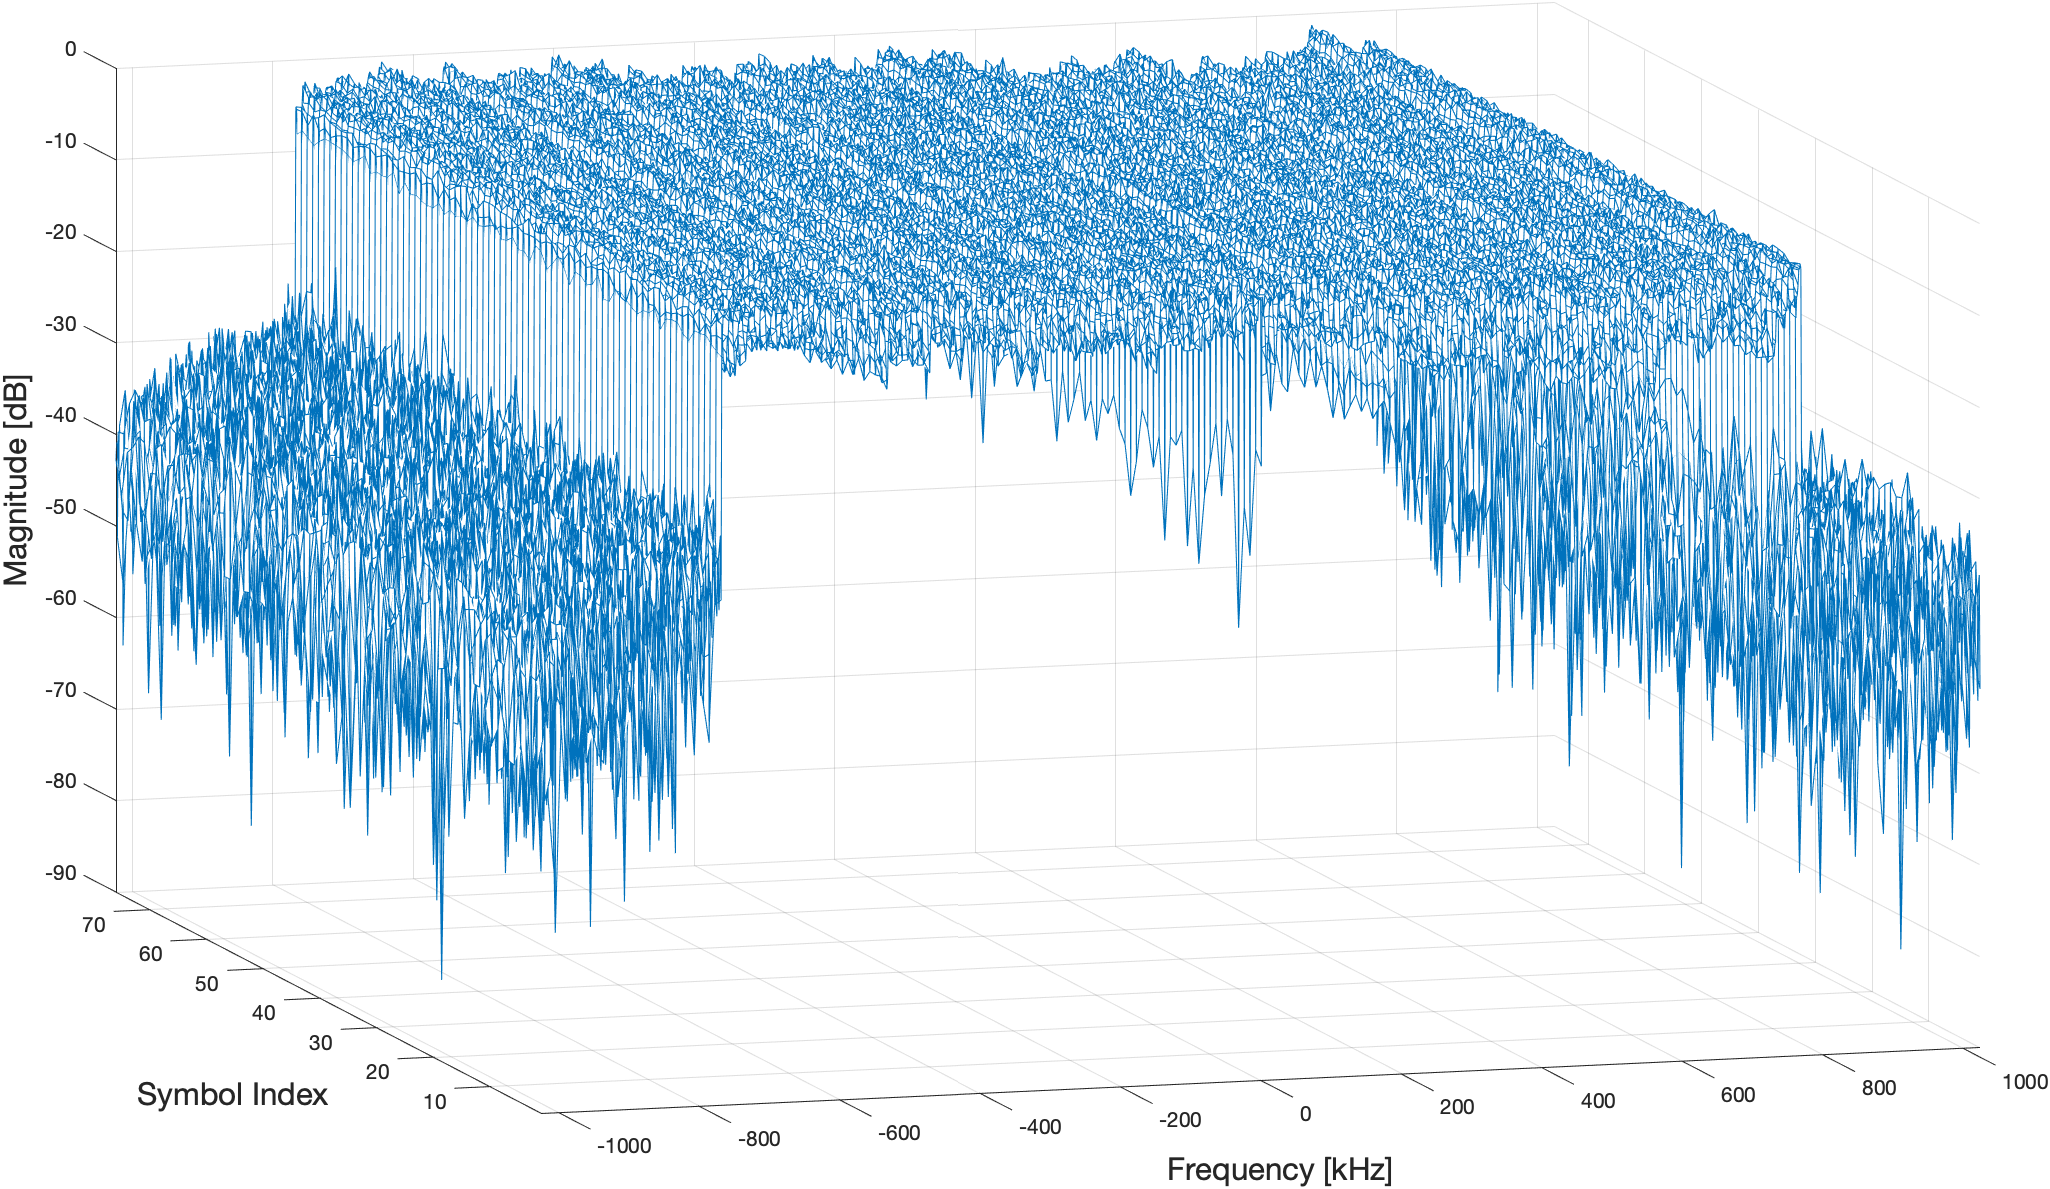
\includegraphics[width=0.9\linewidth]{plots/ofdm-surface-raw.png}
  \caption{Surface plot}
  \label{fig:ofdm-surface-raw}
\end{figure}



\begin{figure}[htbp]
  \centering
  \captionsetup{type=figure}
  \def\svgwidth{\linewidth}
  {\setstretch{0.7} % Line spacing
      \input{../Images/ofdm_demux.pdf_tex}}
  \caption{Illustration of the \texttt{ofdm\_demux} functionality}
  \label{fig:ofdm_demux}
\end{figure}



\subsection{DQPSK Demapping \label{subsect:dab-proc_dqpsk-demap}}

\begin{figure}[htbp]
  \centering
  \begin{subfigure}[t]{0.3\textwidth}
    \centering
    \captionsetup{type=figure}
    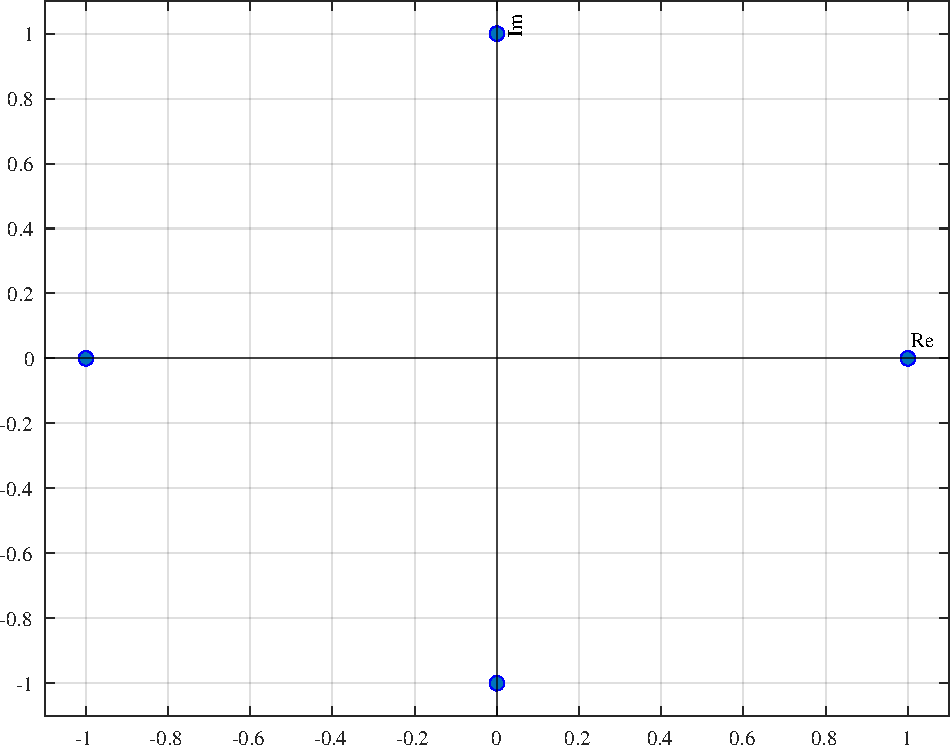
\includegraphics[width=\linewidth]{plots/dqpsk_demap_perfect-1.pdf}
    \caption{}
    \label{fig:dqpsk_demap_perfect-1}
  \end{subfigure}%
  ~ 
  \begin{subfigure}[t]{0.3\textwidth}
    \centering
    \captionsetup{type=figure}
    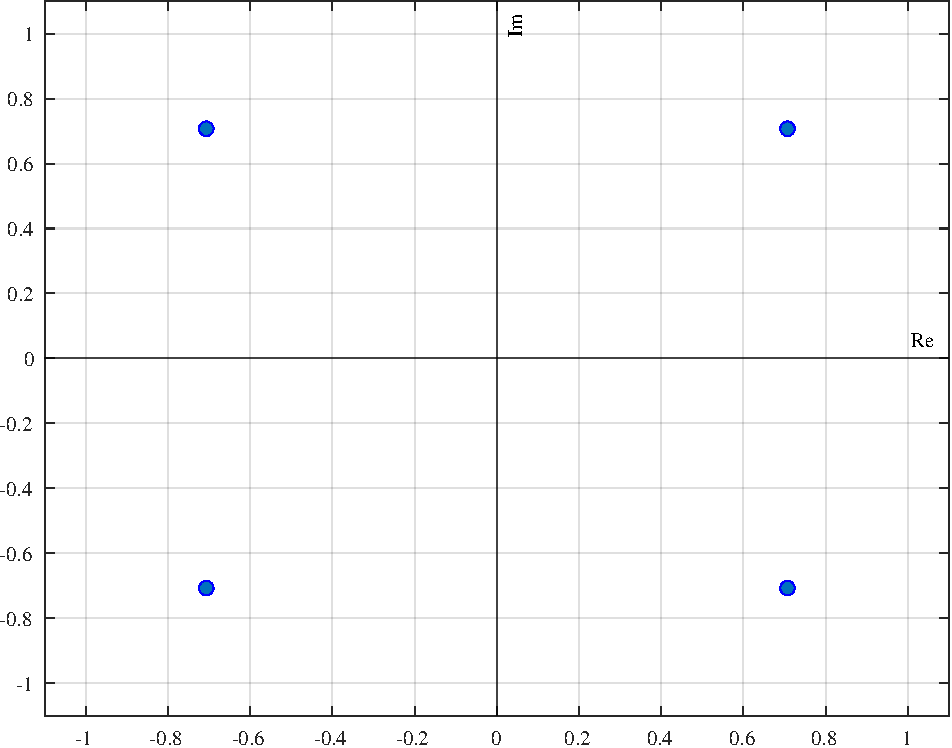
\includegraphics[width=\linewidth]{plots/dqpsk_demap_perfect-2.pdf}
    \caption{}
    \label{fig:dqpsk_demap_perfect-2}
  \end{subfigure}
  ~ 
  \begin{subfigure}[t]{0.3\textwidth}
    \centering
    \captionsetup{type=figure}
    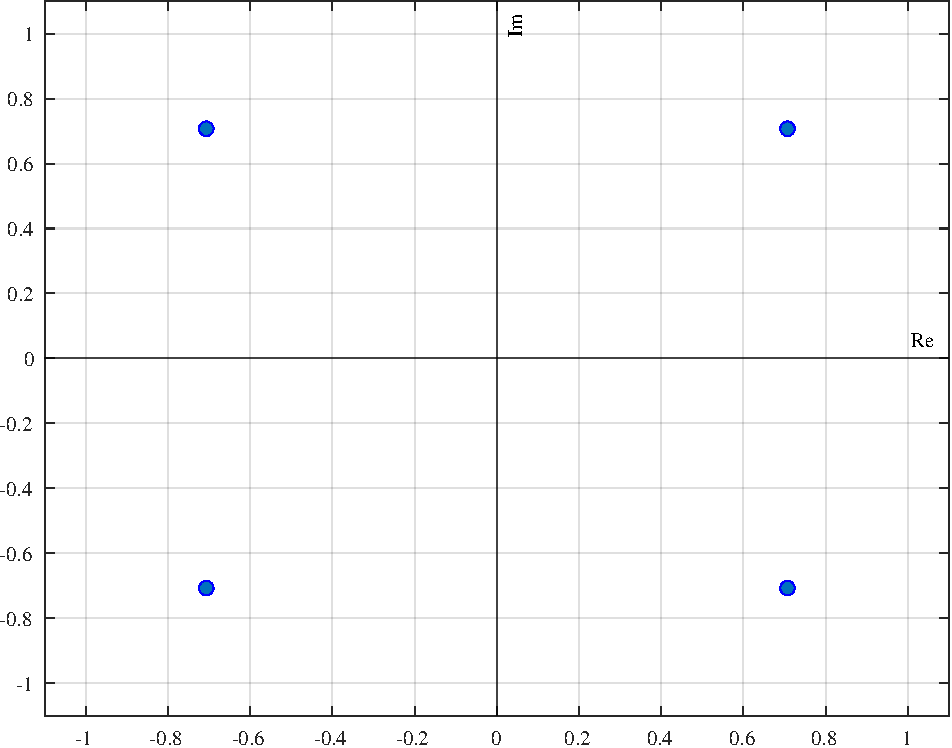
\includegraphics[width=\linewidth]{plots/dqpsk_demap_perfect-2over1.pdf}
    \caption{}
    \label{fig:dqpsk_demap_perfect-2over1}
  \end{subfigure}
  \caption{}
  \label{fig:dqpsk_demap_perfect}
\end{figure}


\begin{figure}[htbp]
  \centering
  \begin{subfigure}[t]{0.3\textwidth}
    \centering
    \captionsetup{type=figure}
    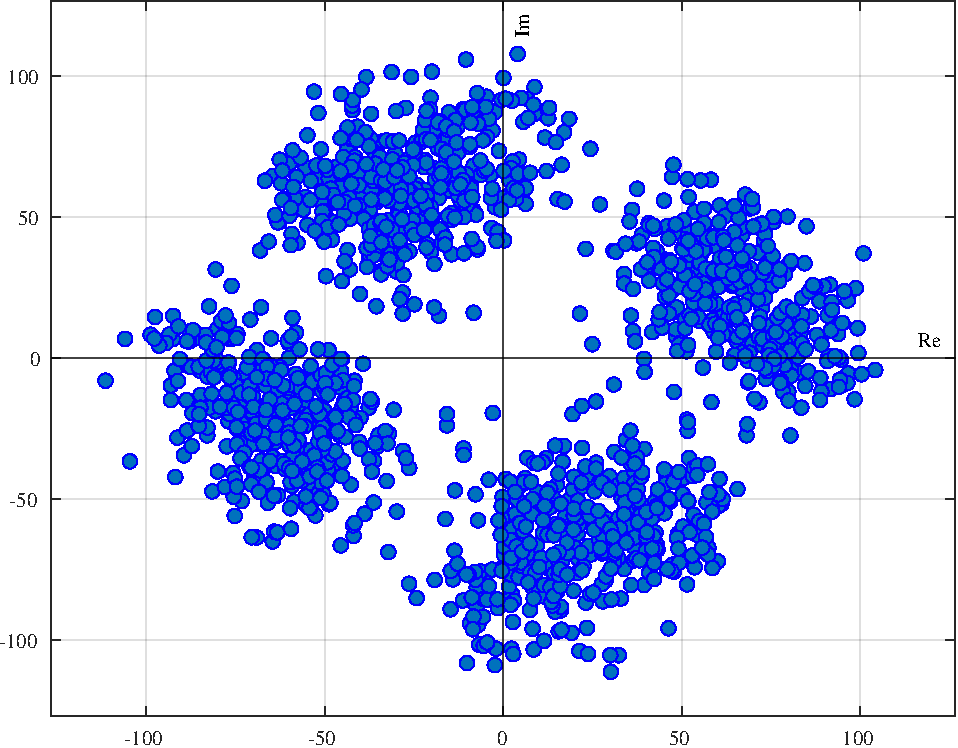
\includegraphics[width=\linewidth]{plots/dqpsk_demap_rtl-1.pdf}
    \caption{}
    \label{fig:dqpsk_demap_rtl-1}
  \end{subfigure}%
  ~ 
  \begin{subfigure}[t]{0.3\textwidth}
    \centering
    \captionsetup{type=figure}
    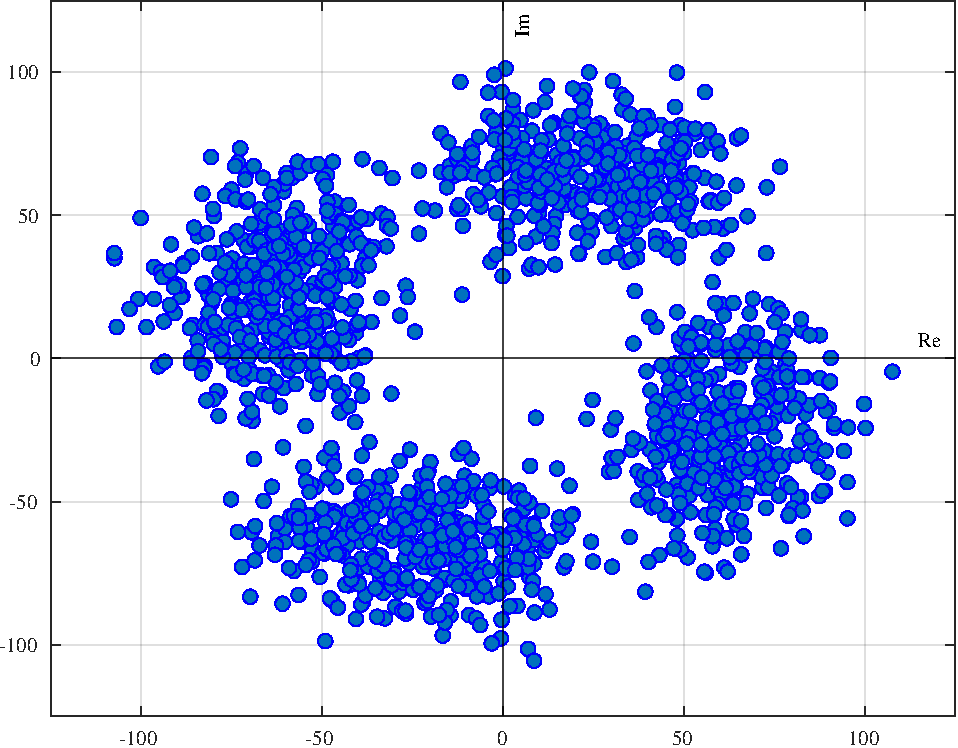
\includegraphics[width=\linewidth]{plots/dqpsk_demap_rtl-2.pdf}
    \caption{}
    \label{fig:dqpsk_demap_rtl-2}
  \end{subfigure}
  ~ 
  \begin{subfigure}[t]{0.3\textwidth}
    \centering
    \captionsetup{type=figure}
    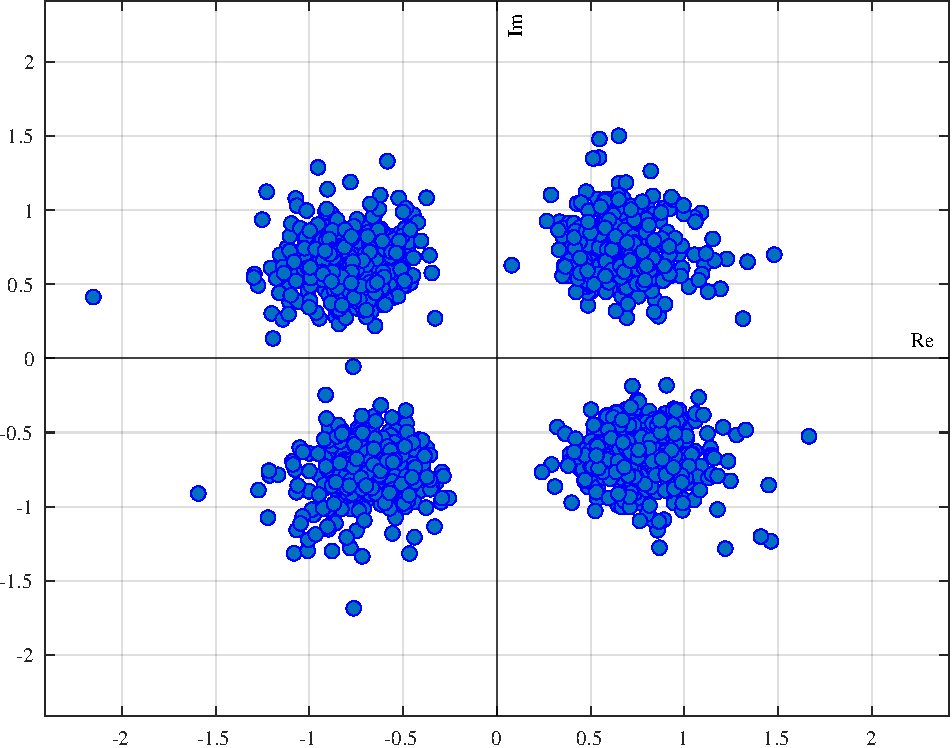
\includegraphics[width=\linewidth]{plots/dqpsk_demap_rtl-2over1.pdf}
    \caption{}
    \label{fig:dqpsk_demap_rtl-2over1}
  \end{subfigure}
  \caption{}
  \label{fig:dqpsk_demap_rtl}
\end{figure}


\begin{figure}[htbp]
  \centering
  \begin{subfigure}[t]{0.3\textwidth}
    \centering
    \captionsetup{type=figure}
    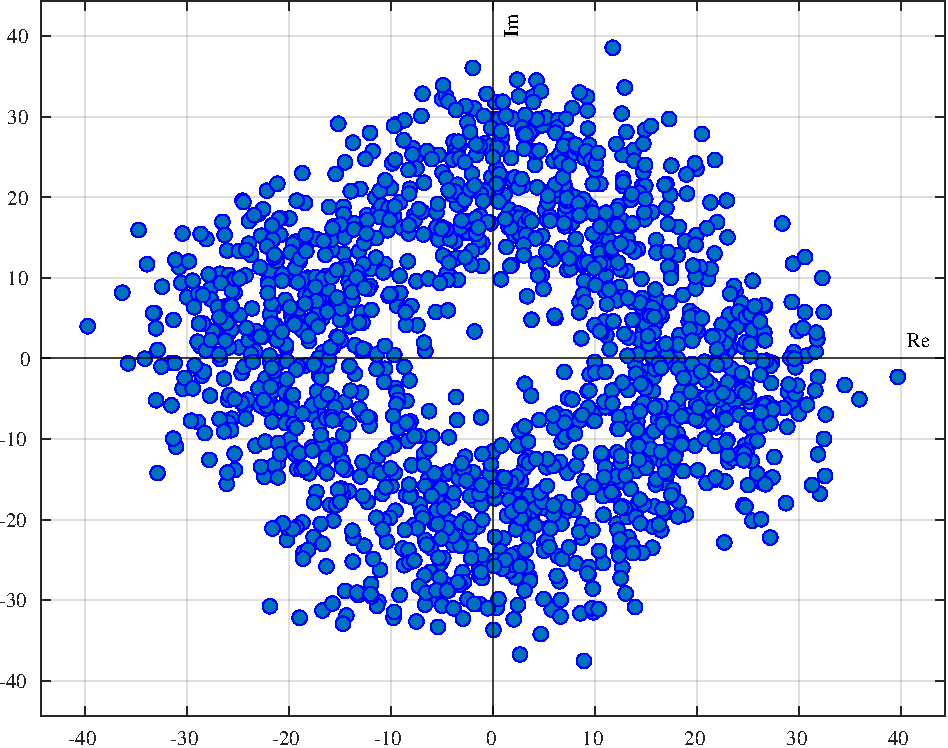
\includegraphics[width=\linewidth]{plots/dqpsk_demap_raw-1.pdf}
    \caption{}
    \label{fig:dqpsk_demap_rtl-1}
  \end{subfigure}%
  ~ 
  \begin{subfigure}[t]{0.3\textwidth}
    \centering
    \captionsetup{type=figure}
    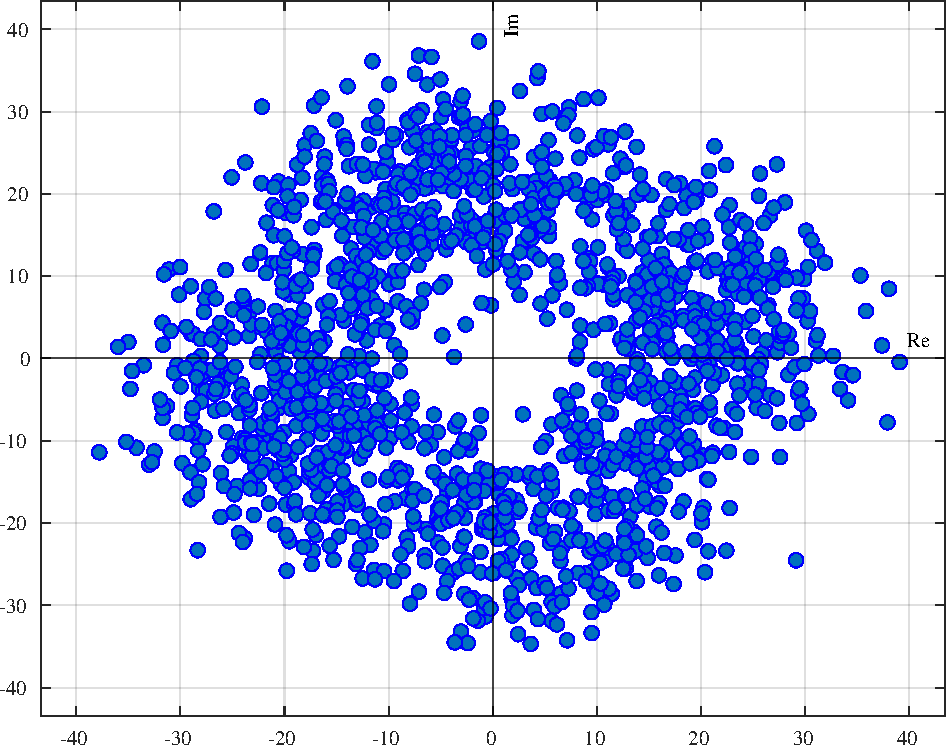
\includegraphics[width=\linewidth]{plots/dqpsk_demap_raw-2.pdf}
    \caption{}
    \label{fig:dqpsk_demap_rtl-2}
  \end{subfigure}
  ~ 
  \begin{subfigure}[t]{0.3\textwidth}
    \centering
    \captionsetup{type=figure}
    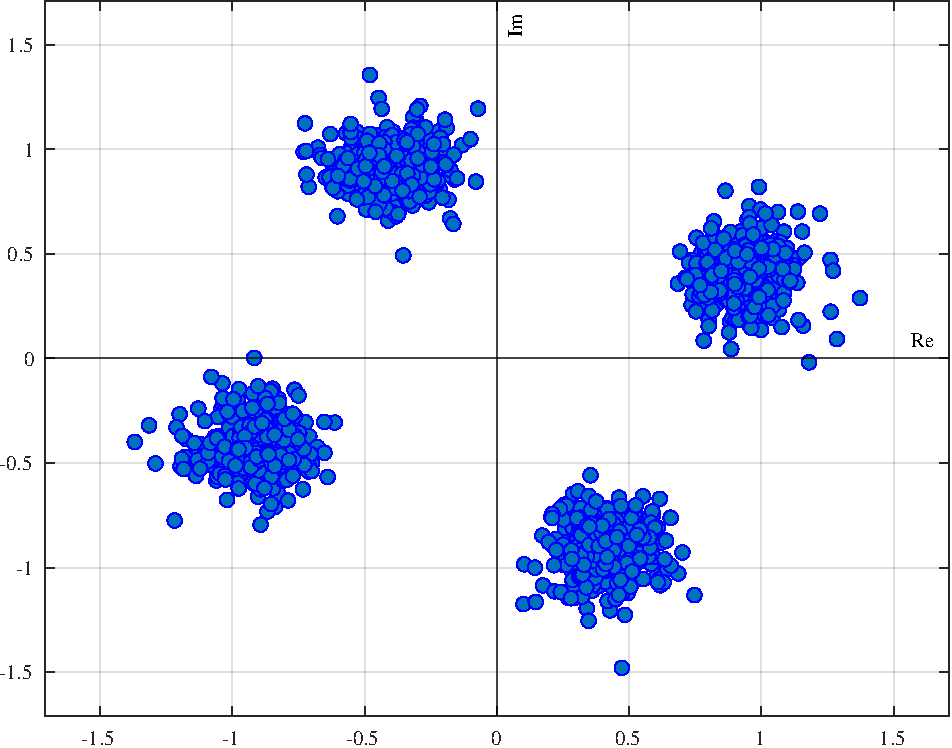
\includegraphics[width=\linewidth]{plots/dqpsk_demap_raw-2over1.pdf}
    \caption{}
    \label{fig:dqpsk_demap_raw-2over1}
  \end{subfigure}
  \caption{}
  \label{fig:dqpsk_demap_raw}
\end{figure}

\begin{figure}[htbp]
  \centering
  \captionsetup{type=figure}
  \def\svgwidth{\linewidth}
  {\setstretch{0.7} % Line spacing
      \input{../Images/dqpsk_demap.pdf_tex}}
  \caption{}
  \label{fig:dqpsk_demap}
\end{figure}


\subsection{Frequency Deinterleaving \label{subsect:dab-proc_freq-deinterleave}}

\subsection{DQPSK Snapping \label{subsect:dab-proc_dqpsk-snap}}

\begin{figure}[htbp]
  \centering
  \captionsetup{type=figure}
  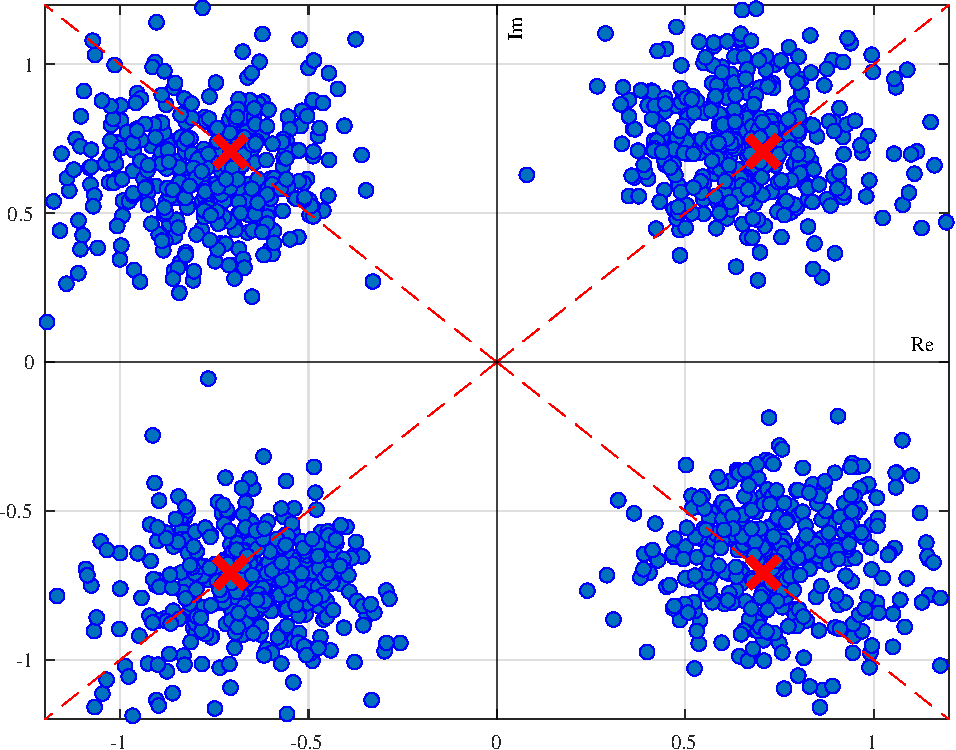
\includegraphics[width=0.8\linewidth]{plots/dqpsk_snap_rtl.pdf}
  \caption{}
  \label{fig:dqpsk_snap_rtl}
\end{figure}

\begin{figure}[htbp]
  \centering
  \captionsetup{type=figure}
  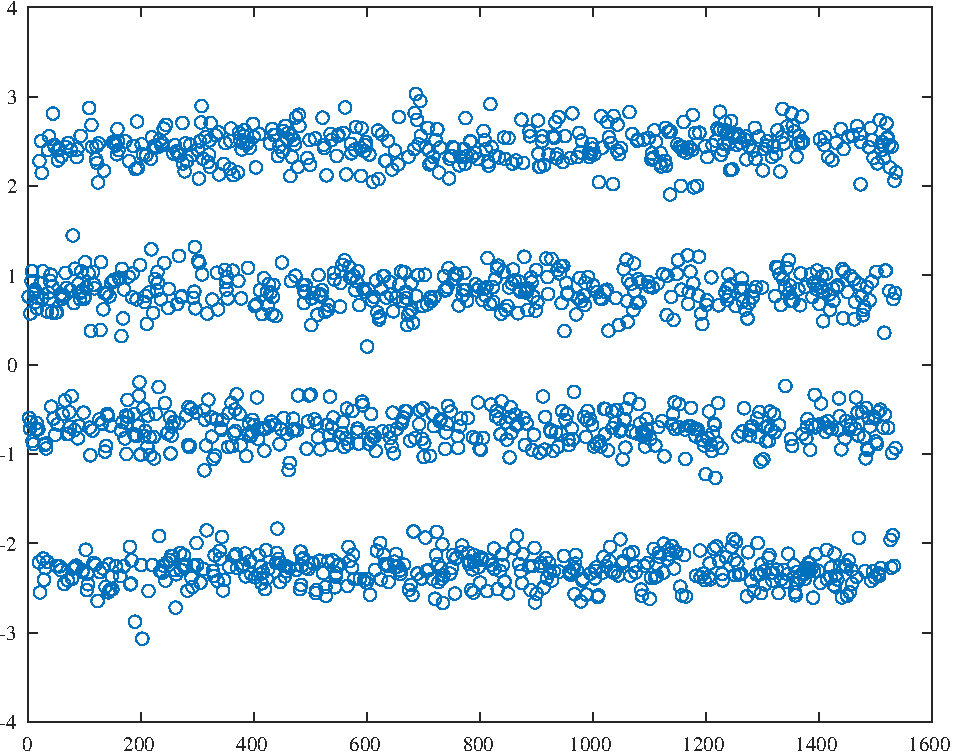
\includegraphics[width=0.8\linewidth]{plots/dqpsk_snap_rtl-alt.pdf}
  \caption{}
  \label{fig:dqpsk_snap_rtl-alt}
\end{figure}

\subsection{Error Correction \label{subsect:dab-proc_error-correct}}

\section{Remodulation \label{sect:dab-proc_remodulate}}

\subsection{Overview}

\begin{figure}[htbp]
    \centering
    \captionsetup{type=figure}
    \def\svgwidth{\linewidth}
    {\setstretch{0.7} % Line spacing
        \input{../Images/BD_Remod_All-embed.pdf_tex}}
    \caption{Block diagram showing demodulation section of processing chain}
    \label{fig:BD_Remod_All}
\end{figure}

\subsection{Frequency Interleaving \label{subsect:dab-proc_freq-interleave}}
\subsection{DQPSK Mapping \label{subsect:dab-proc_dqpsk-map}}
\subsection{OFDM Multiplexing \label{subsect:dab-proc_ofdm-mux}}
\subsection{Symbols Packing \label{subsect:dab-proc_symbols-pack}}

\section{Summary}

% ----------------------------------------------------
\ifstandalone
\bibliography{../Bibliography/References.bib}
\printnoidxglossary[type=\acronymtype,nonumberlist]
\fi
\end{document}
% ----------------------------------------------------